\section{Vertiefungsprojekt: A*-Pfadfindung}

Um besser zu verstehen, wie die A*-Pfadfindung funktioniert (und um etwas Spa� beim Programmieren zu haben), wurde der Algorithmus in Java implementiert. Diese Umsetzung basiert auf einem Online-Artikel von Baeldung\cite{a-star-online}. Die Struktur des Gesamtprojekts und seine Durchf�hrung werden in Kapitel \ref{section:vertiefungs-projekt} erl�utert. 

\begin{figure}[H]
    \centering
    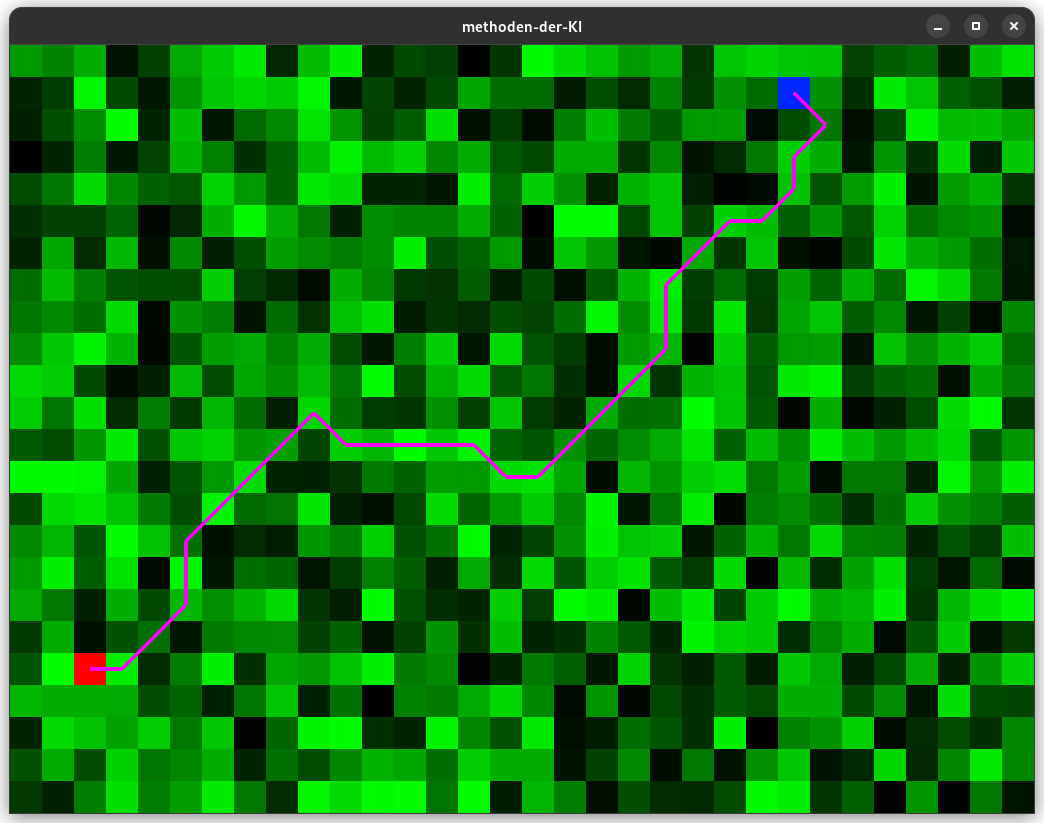
\includegraphics[width=\textwidth]{figures/kap3/a-star-impl.png}
    \caption{Der A*-Pfadfindungs-Screen}
    \label{fig:impl-a-star-pathfinding}
\end{figure}

Bei der Umsetzung wird ein zuf�lliges Terrain in Form von gr�nen Quadraten erzeugt. Je dunkler das Quadrat ist, desto h�her sind die Kosten f�r die Durchquerung des Quadrats. Die Wegfindung beginnt beim roten Quadrat und endet beim blauen Quadrat.

Auf dem A*-Pfadfindungs-Screen des Programms sind die Tastensteuerungen wie folgt:
\begin{itemize}
    \item \textbf{Leertaste:} Erzeugt neues zuf�lliges Terrain und zuf�llige Start- und Endpositionen (Erzeugt eine neue Pfadfindungsaufgabe). 
    \item \textbf{Eingabetaste:} Startet den A*-Pfadfindungsprozess. Der gefundene Pfad wird auf dem SCreen in Form einer hellvioletten Linie angezeigt.
    \item \textbf{Escape-Taste:} Geht zur�ck zum Start-Screen.
\end{itemize}

Es gibt einen Bug im Programm, wodurch manchmal ein Pfad nicht gefunden werden konnte, wenn sich das Ziel am Rand befindet. In diesem Fall wird oben links im Fenster die Meldung ``No traversable route found'' angezeigt.

Der relevante Code f�r das Programm befindet sich in den folgenden Packages (Implementierungscode befindet sich im ``core'' Verzeichnis):
\begin{itemize}
    \item \textbf{de.augsburg.hs.methoden.ki.screens.astar:} Der Code f�r den A-Star-Pathfinding-Screen. Hier kommt der gesamte Code zusammen.
    \item \textbf{de.augsburg.hs.methoden.ki.algorithms.astar:} Allgemeine Implementierung des A*-Wegfindungsalgorithmus.
    \item \textbf{de.augsburg.hs.methoden.ki.algorithms.astar.implementation:} Implementierung des allgemeinen Algorithmus f�r dieses Programm.
    \item \textbf{de.augsburg.hs.methoden.ki.actors.astar:} Enth�lt nur die beiden Actors zum Anzeigen der Start- und Zielquadrate.
\end{itemize}